
%------------------------------------------------------------------------------
% Modelo book de documento. Configurado para papel a4 e fonte de 12 pontos e
% openany evita que seja gerada uma página em branco logo após o índice.
%------------------------------------------------------------------------------
\documentclass[a4paper,12pt,openany]{book}
%------------------------------------------------------------------------------
%  Utiliza idioma Português do Brasil e codificação utf8 para exibir caracteres
%  acentuados.
%------------------------------------------------------------------------------
\usepackage[brazilian]{babel}
\usepackage[utf8]{inputenc}
%------------------------------------------------------------------------------
% Pacotes que acrescentam mais recursos ao texto com notação matemática
%------------------------------------------------------------------------------
\usepackage{amsmath,amsfonts,amssymb}
%------------------------------------------------------------------------------
%  Pacote gráfico para incluir figuras no documento.
%------------------------------------------------------------------------------
\usepackage{graphicx}
%-----------------------------------------------------------------------------
% Pacote para criar minipages de fundo colorido e manipulação de cores em geral
%-----------------------------------------------------------------------------
\usepackage[svgnames]{xcolor} 
%-----------------------------------------------------------------------------
% Define cores de fundo para minipages, layout de código, etc...
%-----------------------------------------------------------------------------
\definecolor{lightblue}{RGB}{173,216,230} 
\definecolor{lightgrey}{RGB}{211,211,211}
\definecolor{greyforcomments}{RGB}{170,170,170}
\definecolor{orange}{RGB}{255,165,0}
%-----------------------------------------------------------------------------
% Define as margens do documento.
%-----------------------------------------------------------------------------
\usepackage{geometry}
\geometry{left=1cm,right=1cm,top=5cm,bottom=2cm}
%-----------------------------------------------------------------------------
% Configura layout para mostrar códigos Java. OBS: Não vai aceitar caracteres
% acentuados nas linhas de comentários dos códigos Java.
%----------------------------------------------------------------------------
\usepackage{listings}
\lstset{
	language=Java,
	basicstyle=\ttfamily\small, 
	keywordstyle=\color{blue}\bfseries,
	stringstyle=\color{orange},
	commentstyle=\color{greyforcomments},
	morecomment=[s][\color{greyforcomments}]{/**}{*/},
	extendedchars=true, 
	showspaces=false, 
	showstringspaces=false, 
	numbers=left,
	numberstyle=\tiny,
	breaklines=true, 
	backgroundcolor=\color{cyan!10}, 
	breakautoindent=true, 
	captionpos=b,
	xleftmargin=0pt,
	tabsize=4
}

%------------------------------------------------------------------------------
% CONVENÇÕES PARA O TEXTO
%
% Variáveis e nomes de métodos são escritos em itálico
%
% Palavras reservadas do Java e classes são escritas em negrito.
%
%------------------------------------------------------------------------------
\begin{document}

\author{Hugo Kaulino Pereira}
\title{Projeto MathPackage}
\date{\today}


\maketitle

%------------------------------------------------------------------------------
%  Cria um índice do documento nomeado como Índice
%------------------------------------------------------------------------------
\renewcommand{\contentsname}{Índice}
\tableofcontents

\newpage

%------------------------------------------------------------------------------
% Define objetivos, requisitos, restrições e relacionamentos deste projeto com
% outros.
%------------------------------------------------------------------------------
\chapter*{Objetivo do Projeto}
\addcontentsline{toc}{chapter}{Objetivo do Projeto}

O objetivo deste projeto é desenvolver pacotes de classes voltadas para problemas matemáticos.
\\
\\
Deverá ter pacotes com bibliotecas de funções, constantes, classes para avaliação de expressões,ferramentas para problemas de análise combinatória e qualquer coisa útil para resolução de problemas matemáticos ou mais diretamente relacionada com Matemática.
\\
\\
Utiliza classes do projeto LocaleToolsPackage e do projeto StringToolsPackage.

\newpage

%*****************************************************************************
% As próximas seções "part" documentam, cada uma, um dos pacotes que constituem
% o projeto.
%*****************************************************************************
 
%------------------------------------------------------------------------------
% Documenta o pacote br.com.hkp.classes.math.
%------------------------------------------------------------------------------
\colorbox{lightblue}{
	
\begin{minipage}{18cm}
	
\part*{Pacote classes.math}
\addcontentsline{toc}{part}{Pacote classes.math}

\paragraph{br.com.hkp.classes.math}

Neste pacote incluem-se classes que lidam genericamente com problemas matemáticos. Como funções - static ou não -  de qualquer tipo, definição de constantes, etc...
\\
\\
São classes para serem utilizadas por outras classes ou aplicações. Não há classes de aplicativos neste pacote. A não ser métodos main() para testes e para fornecer exemplos de uso das próprias classes.

\end{minipage}

}%fim da caixa de texto com fundo colorido

\newpage

%*****************************************************************************
% As próximas seções "chapter" documentam, cada uma, uma das classes que
% constituem o pacote documentado nesta seção "part".
%*****************************************************************************

%------------------------------------------------------------------------------
% Documenta a classe XMath 
%------------------------------------------------------------------------------
\colorbox{lightgrey}{
	
\begin{minipage}{18cm}
	
\chapter*{Classe XMath}
\addcontentsline{toc}{chapter}{Classe XMath}

\paragraph{XMath} - eXtented Math: significando uma espécie de extensão da classe math do pacote java.lang.
\\
\\
O objetivo desta classe é ser uma biblioteca de funções matemáticas diversas,
de preferência implementadas com métodos static. E também definir constantes
matemáticas úteis.

\end{minipage}

}%fim da caixa de texto com fundo colorido

\newpage

%*****************************************************************************
% As próximas seções "section" documentam, cada uma, um dos métodos que
% constituem a classe documetada  nesta seção "chapter".
%*****************************************************************************

%------------------------------------------------------------------------------
% Documenta o construtor XMath
%------------------------------------------------------------------------------
\section*{private XMath()}
\addcontentsline{toc}{section}{XMath()}

Este é o único construtor da classe e é implementado como um método private sem
argumentos. Isso impede que sejam criados objetos da classe XMath, o que não deve mesmo ocorrer, já que esta classe deve ser primordialmente uma biblioteca de funções e constantes matemáticas static.
\\
\\
O corpo do método é vazio; este construtor não faz nada. Sua função é apenas impedir a criação de objetos da classe XMath.


%------------------------------------------------------------------------------
%frac()
%------------------------------------------------------------------------------
\section*{public static double frac(double d)}
\addcontentsline{toc}{section}{frac()}

Retorna a parte fracionaria de um argumento \textbf{double}. Às vezes, ao se 
manipular dados em ponto flutuante, pode ocorrer alguma imprecisao nos
calculos. Como é o caso quando se obtem a parte fracionaria subtraindo-se
o valor do numero de sua representacao inteira. Nesse caso,  de um valor
como 5,97 pode-se obter uma parte fracionaria como 0,966666... Este 
metodo retorna a parte fracionaria de um \textbf{double} ou \textbf{float} sem erros de 
precisão.

\begin{lstlisting}
 return frac( new BigDecimal("" + d) ).doubleValue();
\end{lstlisting}

O método converte o valor \textbf{doubl}e em sua representação \textbf{string}. Em seguida cria um
\textbf{BigDecimal} com essa \textbf{string}, converte o \textbf{BigDecimal} para \textbf{double} e então pega a parte fracionária.
\\
\\
Obs: Peguei este método de outro programador e parece passar nos testes.  

%------------------------------------------------------------------------------
% frac()
%------------------------------------------------------------------------------
\section*{public static BigDecimal frac(BigDecimal bd)}
\addcontentsline{toc}{section}{frac()}

Obtém a parte fracionária de um argumento passado como BigDecimal.
\begin{lstlisting}
 return bd.remainder (BigDecimal.ONE);
\end{lstlisting} 

Obs: O código é de outro programador.

%------------------------------------------------------------------------------
% integ()
%------------------------------------------------------------------------------
\section*{public static double integ(double d)}
\addcontentsline{toc}{section}{integ()}

Retorna a parte inteira de um double ou float.
\begin{lstlisting}
if (d >= 0.0) 
	return Math.floor(d);
else 
	return Math.ceil(d);
\end{lstlisting} 

Note que se o argumento \textit{d} for positivo então a parte inteira é o \underline{maior} inteiro menor ou igual a \textit{d}. Mas se for negativo então a parte inteira é o \underline{menor} inteiro maior ou igual a \textit{d}. Por exemplo: a parte inteira de -3,5 é -3, que é maior que -3,5. Mas a parte inteira de 3,5 é 3, que é menor.

%------------------------------------------------------------------------------
% nPr()
%------------------------------------------------------------------------------
\section*{public static long nPr(int n, int r)}
\addcontentsline{toc}{section}{nPr()}
\label{metodo:nPr01}

Calcula o número de permutações possíveis para n elementos, se cada permutação tiver r elementos. E se r = 0 o método retorna 1, computando apenas uma permutação vazia.
\\
\\
Se r maior que n ou um dos argumentos for negativo, uma exceção é lançada. \textbf{IllegalArgumentException}
\\
\\
Este cálculo é dado pela fórmula $\frac{n!}{(n-r!)}$ e no código é feito por um loop que realiza um produtório de n - r + 1 até n.
$$
\prod_{i = n - r + 1}^{n} i
$$

\begin{lstlisting}
long npr = 1;
for (int p = n - r + 1; p <= n; p++)
	npr *= p;
return npr;
\end{lstlisting} 

%------------------------------------------------------------------------------
% nCPr()
%------------------------------------------------------------------------------
\section*{public static long nCPr(int n, int r)}
\addcontentsline{toc}{section}{nCPr()}
\label{metodo:nCPr01}


\begin{lstlisting}
public static long nCPr(int n, int r)
	throws IllegalArgumentException
{
	/*
	chamada de nPr() verifica se argumentos n e r sao validos
	*/
	return (r == 0) ? 1 : nPr(n,r) / r; 
}//fim de nCPr()
\end{lstlisting} 

Para entender o que é uma permutação circular podemos pensar no problema de existirem 3 cadeiras onde 3 pessoas podem se sentar: João, Paulo e José.
\\
\\
De quantas maneiras diferentes podemos distribuir João, Paulo e José nas 3 cadeiras? De $3!\,=\,6$ maneiras.
\\
\\
Mas se as 3 cadeiras estiverem dispostas ao redor de uma mesa circular, se João se sentar à direita de Paulo, José à direita de João e Paulo à direita de José, então esta seria uma instância de uma permutação circular possível. E haveria 3 maneiras deles se sentarem para resultar nesta mesma permutação circular.
\\
\begin{enumerate}
	\item Paulo $\mapsto$ João $\mapsto$ José
	\item José $\mapsto$ Paulo $\mapsto$ João
	\item João $\mapsto$ José $\mapsto$ Paulo
\end{enumerate}

Nestas 3 disposições João está à direita de Paulo, José à direita de João e Paulo à direita de José.
\\
 Isto é, se são 3 cadeiras, podemos a partir de uma posição qualquer,  "gira-los" 3 vezes (no sentido horário ou anti-horário) para voltarem à configuração original. E a cada vez que são girados uma posição isto produz uma nova permutação simples da disposição das pessoas nas cadeiras. Porém gira-los produz \textbf{a mesma} permutação circular.
\\
\\
Portanto o número de permutações circulares possíveis é o número total nPr de permutações simples dividido pelo número r de elementos em cada permutação. E se r = 0 então é possível apenas uma permutação: a permutação vazia.
$$
\frac{n!}{(n-r)! \cdot r}
$$

Podemos pensar também que cada permutação simples pode ser rotacionada r vezes, e todas estas r permutações simples corresponderão a mesma permutação circular. Então cada permutação circular está associada a r permutações simples. Portanto $ nCPr \cdot r = nPr $ 
\\
\\
Ou
$$
nCPr = \frac{nPr}{r} = \frac{n!}{(n-r)! \cdot r}
$$

\begin{figure}[!h]
	\centering
	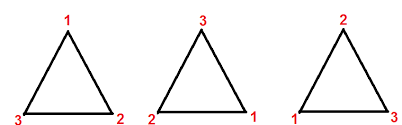
\includegraphics[height=3cm,width=10cm]{figuras/figura1.png}
	\caption{(1,2,3);(3,1,2);(2,3,1) correspondem a uma mesma permutação circular}
	%\label{Rotulo} poderia inserir com o comando rótulo para ref. cruzada.
\end{figure}

%------------------------------------------------------------------------------
% nPr()
%------------------------------------------------------------------------------
\section*{public static long nPr(int[] frequency, int r)}
\addcontentsline{toc}{section}{nPr()}

O método calcula o número de permutações com r elementos possíveis de serem extraídas de um conjunto de n elementos. Mas diferentemente do outro método sobrecarregado nPr(int n, int r), discutido na página ~\pageref{metodo:nPr01}, este permite lidar com um conjunto de n elementos onde existam também elementos repetidos. E se r = 0 o método retorna 1, computando apenas uma permutação vazia.
\\
\\
O argumento \textit{frequency} é um vetor que serve para indicar o número de ocorrências de cada elemento do conjunto de onde se podem extrair as permutações. Se \textit{frequency[0]} é passado com valor 3, por exemplo, isto indicaria que no conjunto há 3 elementos 0. Se \textit{frequency[1]} for passado com valor 0 indicará que não há elemento 1 no conjunto. E assim por diante.
\\
\\
Portanto n é calculado somando todas posições do vetor \textit{frequency}.
\\
\\
Para exemplificar, um conjunto como C = \{0,0,0,2,2,3,4,4,4\} seria representado em \textit{frequency} como \{3,0,2,1,3\}.
\\
\\
\begin{tabular}{|c|c|c|c|c|}
	\hline
	0 & 1 & 2 & 3 & 4 \\
	\hline
	3 & 0 & 2 & 1 & 3 \\
	\hline
\end{tabular}

\begin{itemize}
	\item 3 ocorrências do elemento 0 no conjunto C
	\item 0 ocorrências do elemento 1 no conjunto C
	\item 2 ocorrências do elemento 2 no conjunto C
	\item 1 ocorrências do elemento 3 no conjunto C
	\item 3 ocorrências do elemento 4 no conjunto C
\end{itemize}

 Portanto o conjunto C teria 9 elementos. E 9P3 para este conjunto C, seria o número de permutações possíveis - cada uma com 3 elementos - de serem extraídas de C, considerando que em cada permutação possam ocorrer elementos repetidos também.
\\
\\
Para entender a ideia por trás do algoritmo, imagine que se queira calcular nPr para o conjunto C acima com r = 4. (n seria calculado pelo método para o qual obteria valor 9)
\\
\\
Ao distribuir os três 0s do conjunto C em uma permutação, sobraria apenas uma posição das 4 onde poderia ser inserido mais um elemento de C. Portanto podemos considerar que o número total de permutações onde vão ocorrer 3 0s, é o número de maneiras pelas quais se pode distribuir 3 0s em quatro posições, multiplicado pelo número de maneiras pelas quais se pode distribuir os elementos restantes de C na única posição restante da permutação.
\\
\\
E o número de maneiras pelas quais se pode distribuir 3 elementos iguais em 4 posições é dado por 4C3, ou combinação de 4 em 3. Portanto seria 4C3 multiplicado pelo cálculo de nPr do conjunto C' = \{2,2,3,4,4,4\} para r = 1. Ou seja, o conjunto C menos os elementos 0 que já foram distribuídos de todas as 4C3 formas possíveis. E para cada uma destas formas seria possível extrair nPr permutações do conjunto C' para r = 1 (a posição restante na permutação, já que as outras 3 conteriam 0s)
\\
\\
Se fizermos isso para 3 0s, e depois para 2 0s, e depois para um único 0, somando estes resultados, então teremos o número de permutações possíveis onde ocorre algum elemento 0. Agora bastaria somar a este resultado o número de permutações possíveis - em quatro posições - onde não ocorram nenhum 0, e teremos o nPr (para n = 9 e r = 4) para o conjunto C.
\\
\\
\begin{table}[h]
\begin{center}
	\begin{tabular}{|c||c|c|c|c|}
	\hline
	1 & 0 & 0 & 0 & ?\\
	\hline
	2 & 0 & 0 & ? & 0 \\
	\hline
	3 & 0 & ? & 0 & 0 \\ 
	\hline
	4 & ? & 0 & 0 & 0 \\ 
	\hline
	\end{tabular}
\end{center}
\caption{As 4 distribuições possíveis para 3 0s}
\end{table}
\\ 
\\
A tabela 1 mostra as 4 maneiras possíveis de distribuir os 3 0s do conjunto C em uma permutação de 4 posições. Logo, o número de permutações possíveis onde apareçam 3 0s é 4 multiplicado pelo número de maneiras possíveis de inserir um outro elemento de C na posição vaga indicada pela interrogação. Chamamos este resultado de S1.
\\
\\
\begin{table}[h]
	\begin{center}
		\begin{tabular}{|c||c|c|c|c|}
			\hline
			1 & 0 & 0 & ? & ?\\
			\hline
			2 & 0 & ? & 0 & ? \\
			\hline
			3 & 0 & ? & ? & 0 \\ 
			\hline
			4 & ? & 0 & 0 & ? \\ 
			\hline
			5 & ? & 0 & ? & 0 \\ 
			\hline
			6 & ? & ? & 0 & 0 \\ 
			\hline
		\end{tabular}
	\end{center}
	\caption{As 6 distribuições possíveis para 2 0s}
\end{table}
\\ 
\\
A tabela 2 mostra as 6 maneiras possíveis de distribuir 2 0s do conjunto C em uma permutação de 4 posições. Logo, o número de permutações possíveis onde apareçam 2 0s é 6 multiplicado pelo número de maneiras possíveis de inserir 2 outros elementos de C na nas duas posições vagas indicadas pela interrogação. Chamamos este resultado de S2.
\\
\\
\begin{table}[h]
	\begin{center}
		\begin{tabular}{|c||c|c|c|c|}
			\hline
			1 & 0 & ? & ? & ?\\
			\hline
			2 & ? & 0 & ? & ? \\
			\hline
			3 & ? & ? & 0 & ? \\ 
			\hline
			4 & ? & ? & ? & 0 \\ 
			\hline
		\end{tabular}
	\end{center}
	\caption{As 4 distribuições possíveis para um 0}
\end{table}
\\ 
\\
A tabela 3 mostra as 4 maneiras possíveis de distribuir um único 0 do conjunto C em uma permutação de 4 posições. Logo, o número de permutações possíveis onde apareça um 0 apenas é 4 multiplicado pelo número de maneiras possíveis de inserir outros 3 elementos de C nas posições vagas indicadas pela interrogação. Chamamos este resultado de S3.
\\
\\
O número de permutações possíveis que se quer calcular é S1 + S2 + S3, isto somado ao número de permutações possíveis onde não ocorra nenhum elemento 0. Ou seja, 0 ocorrências para o elemento 0.
\\
\\
E evidentemente o problema de fazer este cálculo (com zero ocorrências para o elemento 0), equivale a resolver o problema de calcular 6P4 para o conjunto C' extraído de C, C' = \{2,2,3,4,4,4\}, onde não há o elemento 0. Portanto este cálculo pode ser resolvido com 4C0 $ \times $ 6P4 calculado para o conjunto C'. Consequentemente a soma S1 + S2 + S3 + 4C0 $ \times $ 6P4 (para 6P4 calculado para o conjunto C') dará o número de permutações possíveis 9P4 para o conjunto C.
\\
\\
O método realiza este cálculo chamando um outro método private nPr(int frequency[], int i, int n, int r), que executa este algoritmo recursivamente.
\\
\\
\begin{lstlisting}
public static long nPr(int[] frequency, int r)
	throws IllegalArgumentException
{
	int n = 0;
	for (int i = 0; i < frequency.length; i++)
	if (frequency[i] < 0) frequency[i] = 0; else n += frequency[i];
	
	if ((r > n) || (r < 0) || (n < 0))
	throw new IllegalArgumentException();
	
	return nPr(frequency,0,n,r);
}//fim de nPr()
\end{lstlisting}

Na linha 11 é chamado o método recursivo. O parâmetro \textit{i}, que o método passa com valor 0, indica que o método recursivo vai começar por tentar distribuir o primeiro elemento de C, o elemento 0, nas posições de cada permutação. Quando \textit{i} é passado como 1 ele calcula as permutações sobre as posições restantes extraindo o elemento 0 do conjunto C. Se i = 2, extrai os elementos 0 e 1, e assim sucessivamente.
\\
\\
O método recursivo é listado abaixo:
\begin{lstlisting}
private static long nPr(int[] frequency, int i, int n, int r)
{ 
	//nao ha mais posicoes disponiveis para incluir elementos de permutacao
	if (r == 0) return 1;
	
	//retornara o calculo de nPr
	long npr = 0;
	
	//numero de elementos que ainda sobrarao, no proximo nivel de recursao,
	//para serem distribuidos pelas posicoes restantes
	n = n - frequency[i]; 
	
	//chama o metodo recursivamente enquanto o numero de elementos que 
	//restarem para serem distribuidos for maior ou igual ao numero de 
	//posicoes disponiveis no proximo nivel de recursao
	for (
	int assignedsElements = Math.min(r, frequency[i]); 
	(assignedsElements >= 0) && (n >= r - assignedsElements);
	assignedsElements--
	)
	
	//nCr() retorna o numero de maneiras que se pode distribuir 
	//<assignedsElements> elementos de permutacao em <r> posicoes
	//Eh multiplicado pelas permutacoes que ainda se pode fazer nas 
	//posicoes restantes com os elementos restantes
	npr += nCr(r, assignedsElements)
	* 
	nPr(frequency, i+1, n, r - assignedsElements);
	
	return npr;
}//fim de nPr()
\end{lstlisting}

Na linha 4 o método checa se r = 0, e nesse caso retorna 1. Pois só há uma permutação possível para r = 0, a permutação vazia. 
\\
\\
No loop for da linha 11 é feito o somatório de todas as permutações possíveis de serem obtidas em que constem algum elemento \textit{i} (cujo número de ocorrência no conjunto C é indicado por \textit{frequency[i]}), e também somado a este resultado uma chamada para o cálculo de nPr com 0 elementos \textit{i}. Ou seja, são somadas todas as permutações possíveis. As que constem elementos \textit{i} e as que não constem.
\\
\\
Mas dois cuidados devem ser tomados para que este loop retorne sempre o resultado correto. O primeiro é que se tivermos elementos \textit{ i}, cujo número de ocorrências em C é \textit{frequency[i]}, e \textit{frequency[i]} for maior que \textit{r}, que é o número de posições disponíveis para distribui-los em uma permutação, obviamente apenas \textit{r} elementos \textit{i} poderão ocupar as \textit{r} posições disponíveis da permutação.
\\
\\
Então a \textit{assingendsElements}, que é o número de elementos \textit{i} que serão distribuídos nas permutações em cada iteração do loop, é atribuído o menor valor entre r e \textit{frequency[i]} na linha 17. Pois se \textit{frequency[i]} maior que r, apenas \textit{r} elementos \textit{i} serão distribuídos pelas \textit{r} posições das permutações.
\\
\\
E também se os \textit{n} de elementos que vão restar em C para serem distribuídos no próximo nível de recursão, for menor que as r - assignedsElements posições que irão restar, então não será possível obter permutações com estes \textit{n} elementos, e portanto o loop não deve executar a iteração onde ocorreria esta chamada recursiva. Na linha 18 a condição booleana $(n >= r - assignedsElements)$ impede que isso ocorra. Pois não executa iterações do loop quando $ n < r - assignedsElements $.
 

%------------------------------------------------------------------------------
% nCPr()
%------------------------------------------------------------------------------
\section*{public static long nCPr(int[] frequency, int r)}
\addcontentsline{toc}{section}{nCPr()}

O método calcula o número de permutações circulares (CP) com r elementos possíveis de serem extraídas de um conjunto de n elementos. Mas diferentemente do outro método sobrecarregado nCPr(int n, int r), discutido na página ~\pageref{metodo:nCPr01}, este permite lidar com um conjunto de n elementos onde existam também elementos repetidos. E se r = 0 o método retorna 1, computando apenas uma permutação vazia. 
\\
\\
Para calcular o número de permutações circulares, com r elementos cada, que se pode extrair de um conjunto com n elementos (denotado por nCPr), dividimos o número de permutações simples que se pode extrair desse mesmo conjunto (também com r elementos cada) por r. Sendo o número destas permutações simples denotado por nPr. De modo que nCPr = $ \frac{nPr}{r} = \frac{n!}{(n-r)! \cdot r} $
\\
\\
Isto porque para cada permutação circular que se possa fazer, existirão r permutações simples associadas que correspondem a esta mesma permutação circular. Portanto 
$ nCPr \cdot r = nPr \text{ , daí }nCPr = \frac{n!}{(n-r)! \cdot r} $
\\
\\
Por exemplo: do conjunto C = \{0, 1, 2\} se pode extrair 6 permutações simples.
\\
\\
\begin{table}[h]
	\begin{center}
		\begin{tabular}{|c||c|c|c|c|c|}
			\hline
			0 & 0 & 1 & 2\\
			\hline
	    	1 & 0 & 2 & 1\\
			\hline
			2 & 1 & 0 & 2\\
			\hline
			3 & 1 & 2 & 0\\
			\hline
			4 & 2 & 0 & 1\\
			\hline
			5 & 2 & 1 & 0\\
			\hline
		\end{tabular}
	\end{center}
	\caption{As 6 permutações simples possíveis}
\end{table}

Mas existem apenas duas permutações circulares possíveis: \{0, 1, 2\} e \{0, 2, 1\}
\\
\\
E note que as permutações 0, 3 e 4 da tabela resultam na mesma permutação circular \{0, 1, 2\}. Enquanto que as permutações 1, 2 e 5 estão associadas à mesma permutação circular \{0, 2, 1\}. Portanto 
$ 3CP3 \cdot 3 = 3P3 \text{ , daí }3CP3 = \frac{3!}{(3-3)! \cdot 3} = 2 $
\\
\\
Porém este raciocínio não pode ser aplicado se no conjunto C de n elementos puder existir repetição de elementos. Como exemplo imagine-se um conjunto C representado pelo vetor \textit{frequency} = [5,4,1], ou seja, o conjunto C = \{0, 0, 0, 0, 0, 1, 1, 1, 1, 2 \}, do qual se queira extrair todas as distintas permutações circulares possíveis com 4 elementos cada. Nesse caso o conjunto $ CP_0 = \{0, 0, 0, 0\} $ é uma permutação possível. Mas essa permutação circular só pode ser associada a uma única (e não 4) permutação  simples com 4 elementos que se possa extrair deste mesmo conjunto C. A saber, a permutação $ PS_0 = \{0, 0, 0, 0\} $. E no caso da permutação circular  $ CP_1 = \{0, 1, 0, 1\} $ existirão apenas duas permutações simples associadas a esta permutação circular:  $ PS_1 = \{0, 1, 0, 1\} $ e  $ PS_2 = \{1, 0, 1, 0\} $
\\
\\
Logo, para este problema, não é verdadeiro que para cada permutação circular estão associadas r permutações simples.
\\
\\
Notamos que para uma permutação circular qualquer (n/d)CPb, onde b = r/d, se pudermos extrair d ou mais subconjuntos de C que sejam iguais ao da permutação (n/d)CPb, então a permutação nCPr formada por d repetições da permutação (n/d)CPb pode ser associada a b = r/d permutações simples nPr.
\\
\\
Chamaremos de permutação circular homogênea uma permutação qualquer formada por sequências de elementos que se repetem. Por exemplo: $ CP_0 = \{0, 0, 0, 0\} $ e  $ CP_1 = \{0, 1, 0, 1\} $ são permutações circulares homogêneas extraídas do conjunto C explicitado acima. Se uma sequência se repete d vezes em uma permutação homogênea então esta sequência tem b = r/d elementos e esta permutação será chamada permutação homogênea de ordem B.
\\
\\
E cada permutação circular homogênea de ordem B está associada a B permutações simples nPr extraídas do conjunto C. Isto é, existirão B permutações simples nPr que resultam nesta mesma permutação circular homogênea. Portanto se existem N permutações homogêneas de ordem B, existem $ N \cdot b = N \cdot \frac{r}{d} $ permutações simples nPr associadas (que correspondem a uma mesma permutação circular).
\\
\\
Para se saber quantas permutações simples correspondem (resultam) a uma mesma permutação homogênea de ordem B, podemos dividir os elementos do vetor \textit{frequency} por d, ou seja, fazer para cada elemento i do vetor \textit{frequency}, frequency[i] / d. Podemos atribuir estes valores calculados às posições de um novo vetor\textit{ frequencyOfSubSet}.
\\
\\
E então calculamos quantas permutações simples (n/d)Pb, cada uma com b elementos, podem ser extraídas do conjunto denotado pelo vetor\textit{ frequencyOfSubSet}. (n/d)Pb dará o número de permutações simples, dentre todas as nPr permutações simples que se pode extrair do conjunto C, que resultam em permutações circulares homogêneas de ordem B. E o número de permutações circulares homogêneas de ordem B associadas a estas permutações simples é dado por (n/d)Pb / b.
\\
\\
Se obtivermos todos os divisores de r ($ d_q, ..., d_2, d_1 $), com $ d_1 = 1 \text{ e }d_q = r $, $ \frac{(n/d_1)Pr}{r} + \frac{(n/d_2)Pb_2}{b_2} + ... + \frac{(n/d_q)P1}{1}$ dará o número nCPr de permutações circulares que se podem extrair do conjunto C, cada uma com r elementos. Sendo que $ \frac{(n/d_1)Pr}{r} $ é o número de permutações \textbf{não} homogêneas. Ou seja, somamos o total de permutações homogêneas com o total de permutações não homogêneas para obter o total de todas as permutações circulares possíveis.
\\
\\
Porém ao se computar $ (n/d_i)Pb_i $ é preciso perceber que se está computando todas as permutações  $ (n/d_j)Pb_j $ onde $ b_j $ seja divisor de $ b_i $. Portanto ao se computar cada $ (n/d_i)Pb_i $ é preciso subtrair deste resultado todos os $ (n/d_j)Pb_j $ já calculados onde $ b_j $ seja divisor de $ b_i $.
\\
\\
Por exemplo: \{0, 1, 2, 0, 1, 2, 0, 1, 2, 0, 1, 2\} é uma permutação circular homogênea de ordem 6, pois a sequência de 6 elementos \{0, 1, 2, 0, 1, 2\} se repete duas vezes. Mas é também uma permutação de ordem 3 onde a sequência \{0, 1, 2\} de 3 elementos se repete 4 vezes. Então ao se computar o número de permutações simples que resultam na permutação circular homogênea \{0, 1, 2, 0, 1, 2, 0, 1, 2, 0, 1, 2\} de ordem 6 percebe-se que esta também é uma permutação de ordem 3, e portanto já foi somada ao total quando se computou (n/4)P3. Daí a necessidade, para obter o resultado correto, que ao se computar cada $ (n/d_i)Pb_i $,  subtrair deste resultado todos os $ (n/d_j)Pb_j $ já calculados onde $ b_j $ seja divisor de $ b_i $. Como exemplo, se r = 12 seus divisores são 1, 2, 3, 4, 6 e 12. Se começamos computando (n/r)P1, depois para (n/6)P2 devemos subtrair deste resultado o valor que foi calculado para (n/r)P1, já que 1 é divisor de 2. O mesmo para (n/4)P3. Para (n/3)P4 devemos subtrair (n/r)P1 e (n/6)P2 e para (n/2)P6 subtraímos (n/r)P1, (n/6)P2 e (n/4)P3.
\\
\\
Finalmente para nP12 subtraímos (n/r)P1, (n/6)P2, (n/4)P3, (n/3)P4 e (n/2)P6.
\\
\\
nCP12 será dado por $ \frac{nP12}{12} + \frac{(n/2)P6}{6} + \frac{(n/3)P4}{4} + \frac{(n/4)P3}{3} + \frac{(n/6)P2}{2} + \frac{(n/12)P1}{1}$
\\
\\
O programa obtém a lista de todos os divisores de r na linha 73. E no loop que se inicia na linha 80 calcula inicialmente (n/r)P1, com \textit{divR} recebendo o valor do primeiro divisor de \textit{r} em\textit{ listOfDivR} e este resultado é armazenado na posição de índice 1 do vetor \textit{mapOfDivR}. Portanto, na verdade, quando \textit{divR} = 1 calculamos (n/r)P1. \textit{divR} é sempre o número de elementos $ b_i $ em $ (n/d_i)Pb_i $. Logo $ divR = \frac{r}{d_i} $
\\
\\
E como $ d_i = \frac{r}{divR} $ na linha 83 calculamos $ \frac{n}{d_i} = \frac{n \cdot divR}{r} $. Como n, número de elementos do conjunto C, é a soma das frequências de cada um destes elementos no conjunto (frequência esta que é passada ao método no vetor \textit{frequency}), $ \frac{n}{d_i} $ é obtido na linha 83 dividindo cada frequency[i] por $ d_i = \frac {r}{divR} $.
\\
\\
Na linha 97 calcula-se $ (n/d_i)Pb_i $ para cada $ b_i $ atribuído à variável divR a cada iteração do loop.
\\
\\
Na linha 102 o método obtém uma lista com todos os divisores de \textit{divR} e na linha 106 remove o próprio \textit{divR} dessa lista. Em seguida, na linha 119, subtrai todas as permutações simples já calculadas para os $ b_j $ divisores de $ b_i = divR $
\\
\\
E como o número de permutações circulares homogêneas que correspondem a estas permutações simples é dado por $ \frac{(n/d_i)Pb_i}{b_i} $, na linha 132 estas permutações são somadas à variável \textit{ncpr}. Exceto na última iteração do loop, quando $ divR = b_i = r $, porque nesta iteração são somadas a $ ncpr $ o total de todas as permutações circulares não homogêneas.
\\
\\
\begin{lstlisting}
public static long nCPr(int[] frequency, int r)
	throws IllegalArgumentException
{
	/*
	Se r = 0 o numero de permutacoes possiveis deve ser retornado como 1.
	representando a permutacao conjunto vazio, ou permutacao vazia. Por
	coerencia com as formulas para outros tipos de permutacao que retornam
	1 quando r = 0.
	*/
	if (r == 0) return 1;
	
	/*
	Calcula o numero n de elementos no conjunto C para o qual sera calculado
	quantas permutacoes circulares podem ser extradidas.
	Se r > n ou r negativo entao nao eh possivel extrair permutacao deste
	conjunto e uma excecao IllegalArgumentException eh lancada.
	*/
	int n = 0;
	for (int i = 0; i < frequency.length; i++)
		if (frequency[i] < 0) frequency[i] = 0; else n += frequency[i];
	
	if ((r > n) || (r < 0)) throw new IllegalArgumentException();
	
	/*
	Ha uma posicao neste array para cada um dos divisores de r. Incluindo
	o 1 e o proprio r. As posicoes cujos indices nao forem divisores de r
	nao sao utilizadas. Quando um arranjo de tamanho r pode ser repartido
	em i grupos de r/i posicoes cada, e cada um destes grupos contiver 
	exatamente a mesma permutacao, chamarei esta permutacao em r de 
	PERMUTACAO HOMOGENEA. Por exemplo, para r = 9, uma permutacao
	[0,1,2,0,1,2,0,1,2] seria uma permutacao homogenea. Pois [0,1,2]
	eh uma permutacao que esta presente nos tres grupos de tres posicoes.
	Uma posicao i do array mapOfDivR terah a funcao de armazenar quantas
	pormutacoes simples em i posicoes (permutacoes nao circulares nPr com r
	= i), sao possiveis de modo que se possa produzir uma permutacao
	homogenea repetindo esta mesma permutacao nos outros grupos de i
	posicoes do arranjo com r elementos.
	Exemplo: para r = 9, i = 3 eh divisor de r. Logo podemos repartir o 
	arranjo de 9 posicoes em 3 com 3 posicoes cada.
	Se frequency fosse passado como [3,3,3] este array do argumento 
	frequency representaria o conjunto C = {0,0,0,1,1,1,2,2,2} de onde se
	quer calcular quantas permutacoes circulares distintas se pode fazer com
	9 elementos cada. Nesse caso se poderia obter 6 permutacoes distintas
	simples (nao circulares) com 3 elementos cada que poderiam produzir
	permutacoes homogeneias em r = 9. Por exemplo, a subpermutacao 
	[0,1,2], extraida do conjunto C = {0,0,0,1,1,1,2,2,2}, pode ser repetida
	em 3 grupos de 3 posicoes em um arranjo de tamanho 9 gerando a seguinte
	permutacao homogeneizada [0,1,2,0,1,2,0,1,2]. Portanto, neste caso, a
	posicao i = 3 de mapOfDivR armazenarah 6, indicadno o numero de
	permutacoes simples que podem ser feitas em 3 posicoes e que possam ser
	replicadas nos outros grupos de 3 posicoes gerando uma permutacao 
	homogenea no arranjo de tamanho 9.
	*/
	long[] mapOfDivR = new long[r+1];
	
	/*
	Este array tem a funcao de representar um subconjunto de C com 
	com n / i elementos, se i divisor de r, para se verificar se podem ser
	dispostos em subpermutacoes de tamanho i que gerem permutacoes 
	homogeneas no arranjo de tamanho r
	*/
	int[] frequencyOfSubSet = new int[frequency.length];
	
	/*
	Retornara o numero de permutacoes circulares
	*/
	long ncpr = 0;
	
	/*
	Um lista ligada com todos os divisores de r ordenada em ordem crescente.
	A lista inclui o 1 (um) e o proprio r.
	*/
	LinkedList<Integer> listOfDivR = allFactors(r);
	
	/*
	Para cada divisor de r (divR), calcula quantas permutacoes simples de 
	divR posicoes sao possiveis de modo que estas gerem um arranjo de 
	tamanho r com permutacao homogenea 
	*/
	for (int divR: listOfDivR)
	{
	
		for (int i = 0; i < frequencyOfSubSet.length; i++)
			frequencyOfSubSet[i] = (frequency[i] * divR) / r;
		
		try
		{
			/*
			Numero de permutacoes simples que se pode fazer em divR posicoes
			que gerem arranjos de tamanho r com permutacao homogenea eh
			armazenada na posicao divR do array mapOfDivR.
			Se nPr() gerar uma excecao IllegalArgumentException entao nao
			ha permutacao possivel de tamanho divR que gere permutacao 
			homogenea no arranjo de tamanho r. Na clausula catch serah
			atribuido 0 a mapOfDivR[divR]
			*/
			mapOfDivR[divR] = nPr(frequencyOfSubSet, divR);
			/*
			Uma lista com todos os divisores de divR. Que obviamente tambem
			sao divisores de r.
			*/
			LinkedList<Integer> sublistOfDivR = allFactors(divR);
			/*
			Remove o proprio divR desta lista.
			*/
			sublistOfDivR.removeLast();
			
			/*
			Subtrai do numero de permutacoes simples atribuidas a 
			mapOfDivR[divR], o numero de permutacoes simples que ja foram
			atribuidas a subarranjos contidos em um arranjo de divR posicoes
			Exemplo: um subarranjo de 4 posicoes que se pode tomar em um
			arranjo de 8 posicoes, tambem pode ser dividido em 2 arranjos de
			duas posicoes cada. Entao para o numero de permutacoes simples
			que se atribuiu ao aubarranjo de 4 posicoes sao descontadas as 
			permutacoes simples possiveis que ja foram calculadas para 
			subarranjos de duas posicoes.
			*/
			for (int dD: sublistOfDivR) mapOfDivR[divR] -= mapOfDivR[dD];
			
			/*
			Adiciona a ncpr quantas permutacores circulares homogeneas
			em particoes identicas de divR elementos, sao possiveis de 
			serem feitas com arranjos de tamanho r
			Mas para divR = r temos o numero de arranjos nao homogeneos.
			Portanto ncpr eh um acumulador que soma todos arranjos do tipo
			homogeneos com todos os nao homogeneos, obtendo ao final do loop
			o numero total de arranjos possiveis com r elementos cada, que
			podem ser extraidos do conjunto C cujos elementos estao 
			indicados no argumento frequency[] passado a este metodo. 
			*/
			ncpr += mapOfDivR[divR] / divR;
		
		}
		catch(IllegalArgumentException e)
		{
			mapOfDivR[divR] = 0;
		}
	
	}//fim do for listOfDivR
	
	return ncpr;

}//fim de nCPr()
\end{lstlisting}

%------------------------------------------------------------------------------
% nCr()
%------------------------------------------------------------------------------
\section*{public static long nCr(int n, int r)}
\addcontentsline{toc}{section}{nCr()}


\begin{lstlisting}
public static long nCr(int n, int r)
	throws IllegalArgumentException
{
	if ((r > n) || (r < 0) || (n < 0))
	throw new IllegalArgumentException();
	
	r = Math.min(n - r, r);
	long ncr = 1;
	long termOfRFatorial = 1;
	
	for (int i = n - r + 1; i <= n; i++)
	{
		ncr *= i;
		while ((termOfRFatorial <= r) && (ncr % termOfRFatorial == 0))
			ncr /= termOfRFatorial++;
	}
	
	return ncr;
}//fim de nCr()
\end{lstlisting}

Esse método calcula a fórmula para o número de combinações de n em r, dada por $ \frac{n!}{(n-r)! \cdot r!} $ de uma maneira eficiente.  A fórmula poderia ser escrita como $ \frac{\displaystyle \prod_{i = n - r + 1}^{n} i}{r!} $, porém se fosse calculado o produtório no numerador e em seguida o fatorial no denominador para então operar a divisão de um pelo outro, poderia ocorrer que o resultado do produtório (o numerador) estourasse até o maior valor possível de representação para um inteiro positivo em \textbf{long}, fazendo o método retornar um valor incorreto.
\\
\\
Para evitar este problema, e também para tornar mais rápido o cálculo, no loop da linha 11, a cada valor parcial obtido no cálculo do produtório e atribuído à variável \textit{ncr}, é verificado se \textit{ncr} é divisível pelo menor termo corrente do fatorial de r, a variável \textit{termOfRFatorial}  (inicializado em 1). Se sim, é feita esta divisão e somado um a \textit{termOfRFatorial}, para que a próxima divisão (quando o valor atribuído a \textit{ncr} permitir), seja feita por 2, depois por 3... sucessivamente até r.
\\
\\
O que ocorre no loop while da linha 14.
\\
\\
Observe-se também que se a + b = n, então $ nCa = nCb $, já que nesse caso $ (n-a)! \cdot b!  = (n-b)! \cdot a! $. Mas o método seria mais eficiente para calcular nCa se $ a < b $, por essa razão a linha 7 atribui a r o mínimo entre r e n - r antes de executar o loop da linha 11.
\\
\\
O número de combinação para r = 0 é 1. Pois essa combinação é o conjunto vazio.


%------------------------------------------------------------------------------
% sum()
%------------------------------------------------------------------------------
\section*{public static int sum(int[] s)}
\addcontentsline{toc}{section}{sum()}

\begin{lstlisting}
public static int sum(int[] s)
{
	int sum = 0;
	for (int i = 0; i < s.length; i++) sum = sum + s[i];
	return sum;
}//fim de sum()
\end{lstlisting} 

Retorna o somatório de todos os elementos de um vetor de int.

%------------------------------------------------------------------------------
% sum()
%------------------------------------------------------------------------------
\section*{public static long sum(long[] s)}
\addcontentsline{toc}{section}{sum()}

\begin{lstlisting}
public static int sum(long[] s)
{
	long sum = 0;
	for (int i = 0; i < s.length; i++) sum = sum + s[i];
	return sum;
}//fim de sum()
\end{lstlisting} 

Retorna o somatório de todos os elementos de um vetor de long.

%------------------------------------------------------------------------------
% sum()
%------------------------------------------------------------------------------
\section*{public static double sum(double[] s)}
\addcontentsline{toc}{section}{sum()}

\begin{lstlisting}
public static double sum(double[] s)
{
	double sum = 0;
	for (int i = 0; i < s.length; i++) sum = sum + s[i];
	return sum;
}//fim de sum()
\end{lstlisting} 

Retorna o somatório de todos os elementos de um vetor de double.

%------------------------------------------------------------------------------
% primeFactors()
%------------------------------------------------------------------------------
\section*{public static LinkedList $<Long>$ primeFactors(long n)}
\addcontentsline{toc}{section}{primeFactors()}

Este método retorna uma lista com todos os fatores primos do inteiro \textit{n} passado como argumento para o método.
\\
\\
Se $ \frac{n}{P_1 \cdot P_2 ... P_i} = 1 $ e $\{P_1,P_2,...,P_i\}$ são primos, então $\{P_1,P_2,...,P_i\}$ são os fatores primos de \textit{n} que serão retornados por este método. Porém se \textit{n} é primo o método retorna uma lista vazia, pois \textit{n} não é fatorável.
\\
\\
Se \textit{n} não tem nenhum fator primo $ \leq \sqrt{n} $ então \textit{n} é primo. Pois suponha que n tenha um divisor primo  $ P > \sqrt{n} $. Nesse caso $\frac{n}{P} = Q < \sqrt{n} $, e portanto Q seria um divisor de n menor que $ \sqrt{n} $. Uma contradição.
\\
\\
Logo, se n não tem divisor menor ou igual que  $ \sqrt{n} $ então n é primo.
\\
\\
Usando este resultado o algoritmo do método fatora o inteiro n. O loop while da linha 26 fatora n ou termina com uma lista vazia \textit{listFactors} se n é primo.
\\
\\
O loop while de linha 33 procura um divisor para n até $ \sqrt{n} $ e se não encontrado está demonstrado que n é primo. Mas quando este loop encontra um divisor este é um fator primo de n que é adicionado à lista \textit{listFactors} na linha 54. A variável n é então dividida por este divisor (\textit{div}), \textit{sqrt} é recalculado para este novo valor de n e é iniciada uma nova iteração do loop da linha 26. Novamente o loop ou encontra mais um fator primo dividindo \textit{}n, ou descobre que o n desta iteração é primo pois \textit{div} foi incrementado até um valor maior que \textit{sqrt}. E se \textit{div} for maior que \textit{sqrt} então a condição da linha é true e o loop é encerrado com break. Note-se que neste caso, se a lista ainda estiver vazia, é porque o argumento n passado para o método é um número primo e portanto o método retorna a lista \textit{listFactors} vazia.

\begin{lstlisting}
public static LinkedList<Long> primeFactors(long n)
	throws IllegalArgumentException
{
	if (n < 1) throw new IllegalArgumentException("Integer < 1: " + n);
	
	/*
	Cria a lista que retornara os fatores primos do argumento n
	*/
	LinkedList<Long> listFactors = new LinkedList<Long>();
	
	/*
	Nao podem existir 2 fatores primos de n maiores que raiz de n. No 
	maximo pode haver 1 fator primo de n maior que raiz de n. Logo, se 
	listFactors estiver vazia e a busca nao encontrar nenhum fator primo
	menor ou igual raiz de n, entao n eh primo. Se listFactors nao estiver
	vazia, entao o corrente valor de n serah o ultimo fator primo do valor
	que foi passado pelo argumento n ao metodo.
	*/
	long sqrt = (long)Math.sqrt(n);
	
	/*
	Inicia tentando dividir n pelo menor primo que eh 2. Divide n 
	sucessivamente por fatores primos encontrados ateh n ser igual a 1.
	*/
	long div = 2;
	while (n > 1) 
	{
		/*
		Procura um divisor primo para o valor corrente de n. O loop termina
		se encontrado o divisor (fator primo) ou se nao for encontrado 
		fator primo menor ou igual a raiz quadrada do valor corrente de n
		*/
		while ( (div <= sqrt) && ((n % div) != 0) )
			div++;
		
		/*
		Se nao for encontrado fator primo menor ou igual a raiz quadrada do
		valor corrente de n, entao o valor corrente de n soh eh divisivel
		por ele mesmo. Logo, se a lista de fatores primos estiver vazia,
		entao o valor corrente de n neste loop eh o valor que foi passado 
		ao paramentro n do metodo e n eh primo. Sendo n primo nao eh 
		fatoravel e a lista eh retornada vazia. Se a lista nao estiver vazia
		entao o valor corrente de n eh o ultimo fator primo do inteiro que
		foi passado ao metodo no pelo parametro n.
		*/
		if (div > sqrt)
		{
			if (listFactors.size() > 0) listFactors.add(n);
			break;
		}
		
		sqrt = (long)Math.sqrt(n);
		n /= div; 
		listFactors.add(div);
	
	}
	return listFactors;
}//fim de primeFactors()
\end{lstlisting} 


%------------------------------------------------------------------------------
% primeFactors()
%------------------------------------------------------------------------------
\section*{public static LinkedList $<Long>$ primeFactors(long n, LinkedList$<Integer>$ listPrimes)}
\addcontentsline{toc}{section}{primeFactors()}

A lógica deste método é idêntica a do anterior de mesmo nome. A diferença é que este método pode receber uma lista de fatores primos que pode ser gerada pela classe br.com.hkp.classes.math.numberstheory.QuickSieve, documentada na página ~\pageref{classe:QuickSieve}, e então em vez de procurar pelos fatores primos incrementando a variável div o método percorre a lista de primos passada no parâmetro listPrimes, tornando a execução mais rápida.

\begin{lstlisting}
public static LinkedList<Long> primeFactors(long n, 
											LinkedList<Integer> listPrimes)
	throws IllegalArgumentException
{
	if (listPrimes == null) return primeFactors(n);
	
	if (n < 1) throw new IllegalArgumentException("Integer < 1: " + n);
	
	LinkedList<Long> listFactors = new LinkedList<Long>();
	
	Iterator<Integer> it = listPrimes.iterator();
	
	long sqrt = (long)Math.sqrt(n);
	
	long div = it.next();
	
	while (n > 1) 
	{
		while ( (div <= sqrt) && ((n % div) != 0) )
		{
			if (it.hasNext()) 
				div = it.next();
			else
				div++;
		}
		
		if (div > sqrt)
		{ 
			if (listFactors.size() > 0) listFactors.add(n);
			break;
		}
		
		sqrt = (long)Math.sqrt(n);
		n /= div; 
		listFactors.add(div);
	
	}
	return listFactors;
}//fim de primeFactors()
\end{lstlisting} 

%------------------------------------------------------------------------------
% allFactors()
%------------------------------------------------------------------------------
\section*{public static LinkedList $<Integer>$ allFactors(int n)}
\addcontentsline{toc}{section}{allFactors()}

Este método retorna uma lista (classe \textit{LinkedList}) com todos os divisores do inteiro n passado como argumento ao método. Incluindo o 1 e o próprio n. A lista é ordenada, com o elemento no nó índice 0 sendo sempre o 1 e o último elemento da lista é sempre o n.

\begin{lstlisting}
public static LinkedList<Integer> allFactors(int n)
	throws IllegalArgumentException
{
	if (n < 1) throw new IllegalArgumentException("Integer < 1: " + n);
	
	/*
	Cria as listas que retornarao os divisores do argumento n
	*/
	LinkedList<Integer> listD = new LinkedList<Integer>();
	LinkedList<Integer> listQ = new LinkedList<Integer>();
	
	int sqrt = (int)Math.sqrt(n);
	
	int d = 1;
	do 
	{
	
		listD.add(d);
		int q = n / d;
		if (d != q) listQ.addFirst(q);
		
		do
		{
			d++;
		}while ( ((n % d) != 0) && (d <= sqrt) );
		
	}while (d <= sqrt);
	
	listD.addAll(listQ);
	
	return listD;

}//fim de allFactors()
\end{lstlisting}

%-----------------------------------------------------------------------------
% Fim da documetação dos métodos da classe. Pula para próxima página.
%------------------------------------------------------------------------------
\newpage

%------------------------------------------------------------------------------
% Documenta o pacote br.com.hkp.classes.math.numberstheory
%------------------------------------------------------------------------------
\colorbox{lightblue}{
	
	\begin{minipage}{18cm}
		
		\part*{Pacote classes.math.numberstheory}
		\addcontentsline{toc}{part}{Pacote classes.math.numberstheory}
		
		\paragraph{br.com.hkp.classes.math.numberstheory}
		
		Neste pacote incluem-se classes que lidam com problemas relacionados com a Teoria dos Números. 
		\\
		\\
		São classes para serem utilizadas por outras classes ou aplicações. Não há classes de aplicativos neste pacote. A não ser métodos main() para testes e para fornecer exemplos de uso das próprias classes.
		
	\end{minipage}
	
}%fim da caixa de texto com fundo colorido

\newpage


%------------------------------------------------------------------------------
% Documenta a classe QuickSieve
%------------------------------------------------------------------------------
\colorbox{lightgrey}{
	
	\begin{minipage}{18cm}
		
		\chapter*{Classe QuickSieve}
		\addcontentsline{toc}{chapter}{Classe QuickSieve}
		\label{classe:QuickSieve}
		
		\paragraph{QuickSieve} - Uma classe para gerar uma lista com todos os números primos contidos em um intervalo de inteiros [2 , n]
		\\
		\\
		Um objeto da classe QuickSieve fornece métodos para gerar uma lista de todos os números primos em um intervalo de 2 até n. A classe implementa uma adaptação do algoritmo conhecido como Crivo de Eratóstenes.
		\\
		\\
		Nesse algoritmo temos uma lista de inteiros no intervalo [2,n] e queremos encontrar todos os números primos neste intervalo. Para isto começamos com o primeiro primo, que é 2, e retiramos da lista todos os múltiplos de 2 (que evidentemente não são primos). O próximo número no intervalo evidentemente será 3, que também é primo. Repetimos o processo com o 3. Note que após realizar este passo, o próximo número na lista será sempre primo, pois não foi divisível por nenhum número antes dele. Se fosse teria sido retirado da lista. Então repetindo este passo para todos os elementos da lista irão restar somente primos.
		\\
		\\
		Porém a eficiência do algoritmo consiste no fato de que não é necessário fazer isto para todos os elementos da lista (os que não foram retirados antes de se chegar a eles por serem múltiplos de algum primo anterior na lista), porque basta continuar este processo até $ \sqrt{n} $. Se fizermos isto até $ \sqrt{n} $ só restarão primos na lista.
		\\
		\\
		A dificuldade em se implementar este algoritmo surge quando se quer encontrar todos os primos até algum valor muito grande. Porque neste caso é preciso alocar grande quantidade de memória para a lista com todos os inteiros de 2 até n. E depois ir se retirando os não primos desta lista.
		\\
		\\
		A classe QuickSieve utiliza algumas estratégias para minimizar o uso de memória e tornar mais rápida a execução do algoritmo. Estas estratégias serão vistas quando forem discutidos os métodos da classe. Mas antes se fazem necessárias algumas demonstrações.
	
	\end{minipage}	
	
}%fim da caixa de texto com fundo colorido

\newpage

\colorbox{lightgrey}{
	
	\begin{minipage}{18cm}
		Se um inteiro n não tiver divisor menor ou igual a $ \sqrt{n} $ implica que n é primo. Pois se n é divisível por $ P_1 > \sqrt{n} \text{ então } \frac{n}{P_1} = P_2 \text{ implica que } \frac{n}{P_2} = P_1 \text{, logo } P_2 \text{ também é divisor de n e } P_2 < \sqrt{n} $
		\\
		\\
		Decorre disso que se não for encontrado um divisor para n menor ou igual a $ \sqrt{n} $ então n só pode ser primo. Portanto qualquer inteiro no intervalo [2, n] ou é primo ou divisível por q $ \leq \sqrt{n} $. Então ao se retirar todos os múltiplos de primos menor ou iguais a raiz de n do intervalo [2, n] só podem restar primos neste intervalo. Esta é a ideia básica do algoritmo do crivo de Eratóstenes.
		\\
		\\
		Também se pode demonstrar que se retirarmos do intervalo [2, i] todos os múltiplos de primos menores que $ \sqrt{i}  $ não restará nenhum múltiplo de $ \sqrt{i} < i  $ no intervalo [2, i]. Pois se $ \sqrt{i} \cdot \sqrt{i} = i \text{ então para qualquer } p \cdot \sqrt{i} < i $  implica que $ p < \sqrt{i} $. Portanto $ p \cdot \sqrt{i}  $  é múltiplo também de p e p é menor que $  \sqrt{i} $ ,  logo $ p \cdot \sqrt{i}  $ já teria sido retirado do intervalo como múltiplo de p antes de ser retirado do intervalo como múltiplo de $ \sqrt{i} $. A consequência desta constatação é que podemos começar a retirar os múltiplos de $ \sqrt{i} $ da lista a partir de i. E não antes, pois provamos que o algoritmo do crivo terá retirado todos os múltiplos de $ \sqrt{i} $ que sejam menores que i antes que se comece a eliminar especificamente os múltiplos de $ \sqrt{i} $ ( No caso de $ \sqrt{i} $ ser primo. ) 
		\\
		\\
		Então se poderia percorrer toda a lista a partir de i, saltando sempre $ \sqrt{i} $ a frente, para retirar da lista todos os múltiplos do primo $ \sqrt{i} $. Que seriam i, $ i + \sqrt{i} $, $ i + 2 \cdot \sqrt{i} $, $ i + 3 \cdot \sqrt{i} $ ... até o fim da lista.
		\\
		\\
		Mas notamos que se $ \sqrt{i} $ é ímpar então i é impar. Logo $ i + k \cdot \sqrt{i} $ quando k é ímpar será sempre par. Mas todos os pares já teriam sido retirados da lista como múltiplos do primo 2, portanto não é necessário visitar os inteiros $ i + k \cdot \sqrt{i} $ ( para valores ímpares de k), pois nenhum destes inteiros (todos pares) poderia ainda estar na lista. Logo os "saltos" a partir de i podem ser de $ 2 \cdot \sqrt{i} $ e não de $ \sqrt{i} $, tornando mais rápida a execução do algoritmo.
		\\
		\\
		Estas ideias simples ( e algumas outras ) serão implementadas no método getPrimes() desta classe para otimização do algoritmo.

 
	
	\end{minipage}

}%fim da caixa de texto com fundo colorido

\newpage

Campos da classe:

\begin{lstlisting}
 /*
O metodo getPrimes() implementa um algoritmo baseado no crivo de Eratostenes
e, para isso, cria um array com os inteiros do intervalo de onde serao 
extraidos os numeros primos. O metodo implementa uma lista duplamente ligada
sobre este array e para facilitar a leitura do codigo sao definidas aqui
algumas constantes uteis na manipulacao desta lista.
*/

/*
Indica a posicao anterior (previa) que esta sendo apontada pelo noh corrente
Pois cada elemento do array <numbers> e um ponteiro para um array de tamanho
2, onde a posicao 0 (PREV) apnonta para o no anterior. E a posicao 1 para o
proximo noh da lista duplamente ligada.
*/
private static final int PREV = 0;

/*Indica que a posicao 1 do array aponta para o proximo noh da lista 
duplamente ligada implementada sobre o array <int numbers[][]>
*/
private static final int NEXT = 1;

/*
Indica que um ponteiro nas posicoes PREV ou NEXT do array numbers [][]
aponta para NULL
*/
private static final int NULL = -1;

/*
Se um noh eh removido da lista seu ponteiro PREV recebe o valor da constante
REMOVED, indicando que nao estah mais na lista.
*/
private static final int REMOVED = -2;

/*
O primeiro valor do array <numbers> eh sempre 3.
*/
private static final int FIRST_NUMBER_ON_ARRAY = 3;

/*
O limite superior do intervalo de onde eh extraida a lista de primos.
*/
private final int lastNumber;

/*
Uma lista ligada que contem todos os numeros primos de um determinado
intervalo de inteiros que se inicia em 2. (O primeiro primo da lista)
*/
private final LinkedList <Integer> list;
\end{lstlisting}

%*****************************************************************************
% As próximas seções "section" documentam, cada uma, um dos métodos que
% constituem a classe documetada  nesta seção "chapter".
%*****************************************************************************

%------------------------------------------------------------------------------
% Documenta o construtor QuickSieve
%------------------------------------------------------------------------------
\section*{public QuickSieve(int n)}
\addcontentsline{toc}{section}{QuickSieve()}

\begin{lstlisting}

public QuickSieve(int n)
	throws IllegalArgumentException, OutOfMemoryError
{
	if (n < 2) throw new
	IllegalArgumentException("Unable to create prime's list.");
	
	lastNumber = n;
	
	/*
	Cria a lista e adiciona o primeiro primo.
	*/
	list = new LinkedList<Integer>();
	list.add(2);
	
	/*
	Se n maior que 2 chama getPrimes() para adicionar mais primos na lista.
	*/
	if (n > 2) getPrimes();

}//fim de QuickSieve()

\end{lstlisting}

No caso do valor do argumento \textit{n} exigir mais memória que a disponível para gerar a lista de primos uma exceção \textbf{OutOfMemoryError} é lançada. Esta exceção pode ser capturada em um bloco catch para que se tente criar um objeto desta classe que gere a lista de primos para um valor menor de \textit{n}.

%------------------------------------------------------------------------------
% Documenta o metodo getPrimes()
%------------------------------------------------------------------------------
\section*{private void getPrimes()}
\addcontentsline{toc}{section}{getPrimes()}

Este é o método que realmente gera a lista de números primos.
\\
\\
O método usa o array bidimensional \textit{numbers} declarado na linha 12 para mapear o intervalo de inteiros de onde será extraída a lista de primos. Porém, para economizar memória e tornar a execução mais rápida, neste array são mapeados apenas os números ímpares do intervalo. Já que todos os pares com exceção do 2 são não primos. E o 2 já foi incluído na lista de primos como o primeiro primo no construtor da classe.
\\
\\
Para isso a linha 8 calcula quantos ímpares existem no intervalo [2 , lastNumber] e armazena este valor em \textit{length}.
\\
\\
A classe ainda implementa dois métodos: private int getIndex(int number) e private int getNumber(int index), que respectivamente associam um índice deste array a um número e um valor a um índice do array. Por exemplo: para o intervalo [2, 10] apenas os ímpares 3, 5, 7 e 9 seriam mapeados no array \textit{numbers}, que deverá então ser criado com as dimensões numbers[4][2].
\\
\\
Para getIndex(3) este método retornaria 0, o índice corresponde a posição do valor 3. E para getNumber(0) retornaria 3, o valor que estaria armazenado na posição 0 do array. Porém o array numbers não armazena os valores dos inteiros já que isto não se faz necessário. getNumber() pode calcular o valor que estaria armazenado em uma posição i qualquer do array numbers. Logo não é preciso desperdiçar memória guardando efetivamente um valor v qualquer em uma posição i qualquer deste array.
\\
\\
O que este array realmente armazena são dois ponteiros, implementando sobre o array uma lista duplamente ligada. Para o exemplo acima, inicialmente a posição 1 ( referente ao valor 5, que virtualmente armazena o ímpar 5) tem o ponteiro PREV apontando para 0 ( posição virtual do ímpar 3) e o seu ponteiro NEXT para a posição 2 ( referente ao 7). Assim cada elemento no array aponta para o seu antecessor e seu sucessor na lista, e desta forma para se "retirar" um elemento não primo do array basta executar o código das linhas 84 a 90.
\\
\\
E os ponteiros desta lista duplamente ligada são inicializados no loop da linha 17. Sendo que o antecessor da posição 0 recebe NULL, assim como o sucessor da última posição do array.
\\
\\
Dessa forma o algoritmo do método retira um não primo da lista manipulando estes ponteiros, de forma semelhante a que se retira um nó de uma lista duplamente ligada convencional. E quando uma posição do array é "retirada" ela é marcada recebendo a constante REMOVED no ponteiro PREV desta posição. O que ocorre na linha 87. Ou seja, numbers[i][PREV]aponta para a posição antecessora (prévia) enquanto o nó i estiver na lista ( o array numbers ), mas armazena a constante REMOVED se este nó i foi "retirado" do array.
\\
\\
Fazendo assim, quando o algoritmo termina de retirar todos os não primos do array, não é preciso percorre-lo em todas as posições para encontrar e listar os números primos ( somente estes não serão marcados como REMOVED ). pois o array já estará na forma de uma lista ligada contendo todos os primos do intervalo, com exceção do 2. Mas o 2 já foi inicialmente inserido no objeto LinkedList que fornecerá a lista com os números primos. 
\\
\\
O loop while da linha 32 visita cada primo da lista, a começar pelo 3, e atribui este valor à variável \textit{number}. Para cada valor de \textit{number} o loop interno for da linha 71 retira todos os múltiplos de number da lista, a começar pela posição $ number^2 $, já que como foi demonstrado na seção documentando a classe QuickSieve, neste ponto do algoritmo todos os múltiplos de number menores que $ number^2 $ já terão sido removidos da lista. Observe que este loop for remove na 1ª iteração $ number^2 $, mas na iteração seguinte ele remove $ number^2  + 2 \cdot number$, sem remover o múltiplo de number $ number^2 + number $. Isso porque 
como demonstrado anteriormente, este número sempre será par e por isto já foi removido da lista que foi criada mapeando apenas os valores ímpares do intervalo.
\\
\\
Ao término do loop while ( que é abortado na linha 43, assim que number assume um valor maior que raiz quadrada de lastNumber) o array numbers[][] será uma lista duplamente ligada com todos os primos do intervalo. E no loop da linha 115 estes valores são despejados finalmente em um objeto LinkedList, que já tem o primo 2 como seu primeiro nó. Esta LinkedList é retornada para quem chamar o método getList() desta classe.

\begin{lstlisting}
private void getPrimes()
{

	/*
	Calcula o tamanho do array para conter apenas os inteiros impares do
	intervalo com <n> inteiros
	*/
	int length = 
		(lastNumber - FIRST_NUMBER_ON_ARRAY + 1 + (lastNumber % 2)) /2;
	
	
	int[][] numbers = new int[length][2];
	
	/*
	Monta uma lista duplamente ligada sobre o array numbers.
	*/
	for (int i = 0; i < numbers.length; i++)
	{
		numbers[i][PREV] = i - 1;
		numbers[i][NEXT] = i + 1;
	}
	numbers[0][PREV] = NULL;
	numbers[numbers.length - 1][NEXT] = NULL;
	
	int index = 0;
	int sqrtOfLastNumber = (int)Math.sqrt(lastNumber);
	
	/*
	Inicia retirando todos os multiplos de 3 da lista. Depois de 5, de 7, e
	assim sucessivamente ateh atingir raiz quadrada de lastNumber.
	*/
	while (numbers[index][NEXT] != NULL)
	{
		/*
		Obtem o inteiro primo referente a posicao index da lista.
		*/
		int number = getNumber(index);
		
		/*
		Se number for maior que a raiz quadrada de lastNumber entao todos 
		os nao primos jah foram retirados da lista e o loop se encerra.
		*/
		if (number > sqrtOfLastNumber) break;
		
		/*
		number eh sempre impar pois a lista eh montada apenas com inteiros
		impares. Se um numero N eh multiplo de number e eh N eh par, entao
		N + 2 * number eh impar. E depois deste o proximo multiplo serah
		par e o seguinte impar, e assim sucessivamente. Logo step visita
		todos os nos que sao multiplos de number mas pulando os pares. Jah
		que os pares jah foram retirados previamente da lista.
		*/
		int step = 2 * number;
		
		/*
		A busca por multiplos do primo number que serao retirados da lista
		pode iniciar em N = number^2. Pois todos os nao primos menores que
		number^2 jah terao sido retirados da lista.
		*/
		int first = number * number;
		
		/*
		O indice de first = number^2 na lista montada no array numbers[][].
		Todos os nos visitados por removingIndex sao retirados da lista.
		*/
		int removingIndex = getIndex(first);
		
		/*
		Retira todos os multiplos de number que ainda constarem na lista.
		*/
		for (int i = first; removingIndex < numbers.length; i += step)
		{
			/*
			Se jah foi retirado numbers[removingIndex][PREV] estah marcado
			como REMOVED
			*/
			if (numbers[removingIndex][PREV] != REMOVED)
			{
				/*
				Faz o no anterior apontar para o posterior e o no posterior
				apontar para o anterior, retirando assim o no apontado por
				removingIndex da lista.
				*/
				int prevNode = numbers[removingIndex][PREV];
				int nextNode = numbers[removingIndex][NEXT];
				
				numbers[removingIndex][PREV] = REMOVED;
				
				numbers[prevNode][NEXT] = nextNode;
				if (nextNode != NULL) numbers[nextNode][PREV] = prevNode;
			}
			
			/*
			Visita o proximo multiplo de number que pode ainda nao estar
			marcado como REMOVED
			*/
			removingIndex = getIndex(i);
			
		}//fim do for i
		
		/*
		Pula para o proximo primo da lista.
		*/
		index = numbers[index][NEXT] ;
	
	}//fim do while
	
	/*
	Ao fim do loop while acima soh restarao primos nao marcados como 
	REMOVED no array numbers[][]. O loop abaixo percorre todos estes nos 
	e adiciona os valores primos em uma LinkedList
	*/
	index = 0;
	
	while (index != NULL)
	{
		list.add(getNumber(index));
		index = numbers[index][NEXT]; 
	}


}//fim de getPrimes()

\end{lstlisting}

%-----------------------------------------------------------------------------
% Fim da documetação dos métodos da classe. Pula para próxima página.
%------------------------------------------------------------------------------
\newpage

%------------------------------------------------------------------------------
% Documenta a classe ExtensibleSieve
%------------------------------------------------------------------------------
\colorbox{lightgrey}{
	
	\begin{minipage}{18cm}
		
		\chapter*{Classe ExtensibleSieve}
		\addcontentsline{toc}{chapter}{Classe ExtensibleSieve}
		\label{classe:ExtensibleSieve}
		
		\paragraph{ExtensibleSieve} - Uma classe para gerar uma lista com todos os números primos contidos em um intervalo de inteiros [2 , n] e que permite posteriormente estender este intervalo com o método appendList(int n)
		\\
		\\
		Esta classe é semelhante à classe QuickSieve discutida na página ~\pageref{classe:QuickSieve}. Porém o método appendList(int n), pág. ~\pageref{metodo:appendList()}, permite estender o intervalo de onde é extraída a lista de primos após um objeto da classe ExtensibleSieve ter sido criado.
		
	\end{minipage}

}%fim da caixa de texto com fundo colorido

\newpage

Campos da classe:

\begin{lstlisting}
/*
A classe implementa um algoritmo baseado no crivo de Eratostenes
e, para isso, cria um array com os inteiros do intervalo de onde serao 
extraidos os numeros primos. O metodo implementa uma lista duplamente ligada
sobre este array e para facilitar a leitura do codigo sao definidas aqui
algumas constantes uteis na manipulacao desta lista.
*/

/*
Indica a posicao anterior (previa) que esta sendo apontada pelo noh corrente
Pois cada elemento do array <numbers> e um ponteiro para um array de tamanho
2, onde a posicao 0 (PREV) aponta para o no anterior. E a posicao 1 para o
proximo noh da lista duplamente ligada.
*/
private static final int PREV = 0;

/*Indica que a posicao 1 do array aponta para o proximo noh da lista 
duplamente ligada implementada sobre o array <int numbers[][]>
*/
private static final int NEXT = 1;

/*
Indica que um ponteiro nas posicoes PREV ou NEXT do array numbers [][]
aponta para NULL
*/
private static final int NULL = -1;

/*
Se um noh eh removido da lista seu ponteiro PREV recebe o valor da constante
REMOVED, indicando que nao estah mais na lista.
*/
private static final int REMOVED = -2;

/*
O primeiro numero (sempre impar) mapeado no array numbers[][]
*/
private int firstNumber;

/*
O limite superior do intervalo de onde eh extraida a lista de primos.
*/
private int lastNumber;

/*
A raiz quadrada de lastNumber
*/
private int sqrtOfLastNumber;

/*
Aponta para o indice do primeiro elemento da lista criada no array 
numbers[][]. Inicialmente este indice eh 0, mas se o elemento na primeira
posicao for retirado por ser nao primo, entao pointerToList ira apontar 
para o sucessor deste numero. E, novamente, se este for retirado da lista
entao pointerToList apontarah para o seu sucessor. De modo que pointerToList
sempre aponta para o primeiro noh da lista implementada sobre o array
numbers[][] que eh declarado e criado no metodo appendList(int)
*/
private int pointerToList;

/*
Uma lista ligada que contem todos os numeros primos de um determinado
intervalo de inteiros que se inicia em 2. (O primeiro primo da lista)
*/
private final LinkedList <Integer> list;
\end{lstlisting}

%------------------------------------------------------------------------------
% Documenta o metodo appendList()
%------------------------------------------------------------------------------
\section*{public void appendList(int n)}
\addcontentsline{toc}{section}{appendList()}
\label{metodo:appendList()}

O método appendList() pode criar uma lista com os primos existentes no intervalo [2 , n] quando executado pelo construtor da classe, ou estender o intervalo em N inteiros e sucessivamente acrescentando os primos contidos nesta extensão à lista de primos. Tal lista é retornada pelo método getList() da classe.
\\
\\
A linha 6 do método testa se list.size() == 1 para saber se o método está sendo chamado do construtor, neste caso para criar a lista inicial, ou de um objeto da classe para estender uma lista já existente do objeto. 
\\
\\
Se a variável \textit{creatingNewList} for true o método foi chamado do construtor. E deve então ser gerada uma lista de todos os primos entre 3 e n. Sendo n o argumento que foi passado ao construtor como sendo o limite superior do intervalo de onde deve ser extraída a lista de números primos. Se for false este intervalo será estendido em n inteiros. Por exemplo, se o construtor foi chamando com o argumento 100, como new ExtensibleSieve(100), então é inicialmente gerada uma lista com todos os primos de 2 até 100. Se sequentemente o método appendList for chamando com o argumento 50 então esta lista seria estendida para conter todos os primos existentes entre 2 e 150.
\\
\\
Na linha 70 é determinado se a lista deve ser estendida. Neste caso são utilizados os primos já contidos no campo \textit{list} para retirar todos os múltiplos destes do array \textit{numbers}, e para isso, como já demonstrado na documentação da classe QuickSieve,
é necessário prosseguir apenas até a raiz quadrada do limite superior do intervalo, armazenada no campo \textit{srqtOfLastNumber} na linha 43 do método. Porém se todos os primos em \textit{list} forem menores que \textit{srqtOfLastNumber} o algoritmo prossegue retirando os múltiplos dos primos contidos (mapeados) no próprio array\textit{ numbers[][]} enquanto não for encontrado um primo maior que \textit{srqtOfLastNumber}. E esta tarefa é delegada ao método getPrimes() chamado na linha 119.


\begin{lstlisting}
public void appendList(int n)
	throws OutOfMemoryError
{
	if (n < 1) return;
	
	boolean creatingNewList = (list.size() == 1);
	
	/*
	Se appendList() foi chamado pelo construtor list.size() == 1.
	*/
	if (creatingNewList)
	{
		firstNumber = 3;
		lastNumber = n;
	
	}
	else //senao a lista jah foi criada e serah estendida por appendList()
	{
		/*
		Se lastNumber eh par soma 1. Se eh impar soma 2. Pois firstNumber
		eh e primeiro numero no array numbers que soh mapeia numeros impares
		Logo firstNumber deve ser impar.
		*/
		firstNumber = lastNumber + 1 + (lastNumber % 2);
		/*
		Estende o intervalo de onde sao extraidos os primos em mais n 
		inteiros.
		*/
		lastNumber += n;
		
		/*
		Se o argumento n eh passado como 1, firstNumber pode ser calculado
		como maior que lastNumber se lastNumber for par. Mas como par nao 
		eh primo essa extensao do intervalo nao irah acrescentar nenhum 
		numero primo a lista, entao o metodo simplesmente eh abortado aqui.
		E apenas o campo lastNumber eh atualizado, somando-se n a este.
		Ou seja, somando-se 1, porque neste caso n igual a 1.
		*/
		if (firstNumber > lastNumber) return;
		
	}//fim do if else
	
	sqrtOfLastNumber = (int)Math.sqrt(lastNumber);
	
	/*
	Calcula o tamanho do array para conter apenas os inteiros impares do
	intervalo 
	*/
	int length = 
		(lastNumber - firstNumber + 1 + (lastNumber % 2)) /2;
	
	int[][] numbers = new int[length][2];
	
	/*
	Monta uma lista duplamente ligada sobre o array numbers.
	*/
	pointerToList = 0;
	for (int i = 0; i < numbers.length; i++)
	{
		numbers[i][PREV] = i - 1;
		numbers[i][NEXT] = i + 1;
	}
	numbers[0][PREV] = NULL;
	numbers[numbers.length - 1][NEXT] = NULL;
	
	/*
	Estende a lista atual se appendList() nao estiver sendo chamado pelo
	construtor da classe.
	*/
	if (! creatingNewList )
	{
		ListIterator<Integer> it = list.listIterator(1);
		
		while ( it.hasNext() )
		{
			int prime = it.next();
			
			/*
			Se prime for maior que a raiz quadrada de lastNumber entao todos 
			os nao primos jah foram retirados da lista e o loop se encerra.
			*/
			if (prime > sqrtOfLastNumber) break;
			
			/*
			Calcula qual eh o primeiro multiplo de prime presente no array
			numbers[][]. Mas se este multiplo for par entao firstMultiple
			recebe o proximo multiplo de prime depois deste. Pois o array
			numbers[][] nao mapeia pares, jah que nao ha pares primos alem 
			do 2. Porem se este numero for menor que o quadrado de prime,
			entao a busca por multiplos de prime para serem eliminados da 
			lista se iniciarah em prime^2
			*/
			int firstMultiple = getNumber(pointerToList);
			int q = firstMultiple / prime;
			if ( (q * prime ) < firstMultiple )
				firstMultiple = q * prime + prime;
			
			if ((firstMultiple % 2) == 0) firstMultiple += prime;
			
			int primePower2 = prime * prime;
			
			if (firstMultiple < primePower2) firstMultiple = primePower2;
			
			/*
			Remove todos os multiplos deste primo do array numbers[][]
			*/
			removeMultiples(firstMultiple, 2 * prime, numbers);
			
		}//fim do while
		
	}//fim do if
	
	/*
	Como sqrtOfLastNumber eh campo da classe eh enxergada tambem em 
	getPrimes(). Portanto se este metodo jah tiver extraido todos os nao
	primos do array numbers, o metodo getPrimes() encerra sem acrescentar
	nenhum primo a lista list.
	*/
	getPrimes(numbers);

}//fim de appendList()
\end{lstlisting}

%-----------------------------------------------------------------------------
% Fim da documetação dos métodos da classe. Pula para próxima página.
%------------------------------------------------------------------------------
\newpage

%------------------------------------------------------------------------------
% Documenta o pacote br.com.hkp.classes.math.strings
%------------------------------------------------------------------------------
\colorbox{lightblue}{
	
	\begin{minipage}{18cm}
		
		\part*{Pacote classes.math.strings}
		\addcontentsline{toc}{part}{Pacote classes.math.strings}
		
		\paragraph{br.com.hkp.classes.math.strings}
		
		Neste pacote incluem-se classes que lidam genericamente com problemas matemáticos relacionados de alguma forma a cadeias de caracteres. Como por exemplo o problema de analisar e avaliar uma string de caracteres representando uma expressão algébrica.
		\\
		\\
		São classes para serem utilizadas por outras classes ou aplicações. Não há classes de aplicativos neste pacote. A não ser métodos main() para testes e para fornecer exemplos de uso das próprias classes.
		
	\end{minipage}
	
}%fim da caixa de texto com fundo colorido

\newpage

%*****************************************************************************
% As próximas seções "chapter" documentam, cada uma, uma das classes que
% constituem o pacote documentado nesta seção "part".
%*****************************************************************************

%------------------------------------------------------------------------------
% Documenta a classe ToPosfix
%------------------------------------------------------------------------------
\colorbox{lightgrey}{
	
	\begin{minipage}{18cm}
		
		\chapter*{Classe ToPosfix}
		\addcontentsline{toc}{chapter}{Classe ToPosfix}
		
		\paragraph{ToPosfix} - O construtor recebe como argumento uma string representando uma expressão matemática na forma usual infixa e, depois de fazer a análise léxica da expressão, gera uma estrutura de dados representando esta mesma expressão porém na forma posfixada. Também conhecida como notação polonesa reversa.
		\\
		\\
	
		
	\end{minipage}
	
}%fim da caixa de texto com fundo colorido

\newpage

%*****************************************************************************
% As próximas seções "section" documentam, cada uma, um dos métodos que
% constituem a classe documetada  nesta seção "chapter".
%*****************************************************************************

%------------------------------------------------------------------------------
% Documenta o metodo verifySyntax()
%------------------------------------------------------------------------------
\section*{private void verifySyntax()}
\addcontentsline{toc}{section}{verifySyntax()}

Verifica se a expressão é sintaticamente correta.
\\
\\
Esta providência tem que ser tomada pelo construtor da classe antes de criar a lista posfixa com os tokens da expressão.
\\
\\
A expressão é analisada conforme mostra o gráfico na figura ~\ref{figura:diagrama}. Os retângulos verdes no centro são os dois estados que o método pode assumir: waiting operand e waiting operator.
\\
\\
Em cada um destes estados os tokens lidos na expressão podem ser:

\begin{itemize}
	\item Operador
	\begin{itemize}
		\item PREFIXO
		\item INFIXO
		\item POSFIXO
		\item Menos unário (caso especial)
	\end{itemize}
	\item Operando
	\begin{itemize}
		\item Variável
		\item Literal
	\end{itemize}
	\item Parênteses de abertura 
	\item Parênteses de fechamento
	\item Fim da expressão
\end{itemize}

Na figura ~\ref{figura:diagrama} a ocorrência destes tokens é representada por círculos azuis. Quando um token inesperado é lido isto configura um erro de sintaxe na expressão e o método lança uma exceção \textit{SyntaxErrorException} sinalizando qual token provocou o erro, seu posicionamento na expressão e uma mensagem declarando o tipo de erro de sintaxe. No diagrama estes casos estão representados por círculos azuis com a moldura em vermelho, que levam a emissão das mensagens de erro exibidas nos retângulos com cantos arredondados em laranja, e subsequentemente ao encerramento da execução do método.
\\
\\
Quando é um token esperado é representado por um círculo azul com moldura verde. E então o método toma a ação relativa a este token e pode ou não mudar de estado.
\\
\\
O círculos azuis com moldura preta representam tokens que podem ou não ser válidos, dependendo do que o método checar após a leitura do token. Por exemplo: no estado waiting operand um token representando o sinal de menos ( - ) poderia ser o operador infixo de subtração. Mas poderia também ser o operador prefixo de menos unário (que multiplica seu operando por -1). No primeiro caso seria um erro de sintaxe ( receber um operador infixo quando se espera um operando ), mas no segundo este token seria uma ocorrência válida.
Desse modo se o token (-) for lido no estado waiting operand é assumido ser um sinal de menos unário, e é sintaticamente correto desde que o token anterior a ter sido lido também não tenha sido um outro sinal de menos.
\\
\\
Quando um token menos unário é reconhecido na expressão o seu identificador deve ser trocado pelo identificador de menos unário (que não é o sinal de menos!), porque cada operação tem seu próprio objeto que pertence a uma classe que implementa a interface Operation, e este objeto é localizado (tanto para realizar a operação matemática quanto para fornecer informações sobre o tipo de operação) exatamente pela string (ou caractere) que o identifica na expressão matemática. De modo que não podem haver dois tipos de operações distintas com o mesmo identificador.
\\
\\
O controle sobre a ocorrência legal de parênteses na expressão é feito pela variável \textit{countParenthesis}, que é incrementada toda vez que um parênteses de abertura é lido e decrementada quando um parênteses de fechamento é encontrado. Portanto esta variável não pode nunca assumir valor negativo, o que configuraria um parênteses de fechamento sem o seu correspondente de abertura. E também não pode ser diferente de 0 quanto o método termina de analisar o campo expression (a string com a expressão matemática passada ao construtor da classe ToPosfix). Porque neste caso indicaria mais parênteses de abertura que de fechamento na expressão.
\\
\\
Se este método terminar sem lançar uma SyntaxErrorException a expressão é sintaticamente válida e um objeto da classe pode converte-la para formato posfixo por intermédio do método buildPosfixList().


\begin{lstlisting}
private void verifySyntax()
throws SyntaxErrorException
{
	/*
	Se expression contiver sinais de menos sobrecarregados com a funcao de
	menos unario entao estes caracteres precisam ser trocados pelo caractere
	correto para menos unario definido na classe Neg. Neste caso a troca 
	sera feita em expressionCopy e ao fim deste metodo expressionCopy sera
	atribuida a expression para atualizar este campo com as trocas feitas em
	expressionCopy
	*/
	char[] expressionCopy = expression.toCharArray();
	
	/*
	Conta quantos tokens foram lidos. Essa informacao eh necessaria para
	detectar o erro sintatico de dois operadores menos consecutivos em 
	expression. 
	*/
	int countToken = 0;
	/*
	Esta variavel eh comarada com countToken no loop while para verificar se
	foram lidos dois operadores de subtracao consecutivos.
	*/
	int indexOfLastMinusSignal = -1;
	
	String token;
	/*
	Esse indice varre cada caractere em expression durante o loop while
	*/
	int i = 0;
	
	/*
	A variavel countParenthesis eh inicializada aqui em valor zero e
	eh incrementada cada vez que um parenteses de abertura eh lido. Eh
	decrementada quando um parenteses de fechamento eh lido. Se ficar 
	negativa durante o loop indica que ha um parenteses de fechamento
	sem um correspodente de abertura. Se estiver positiva ( maior que 0 )
	ao termino do loop, indica que ha mais parenteses de abertura que de
	fechamento na expressao.
	*/
	int countParenthesis = 0;
	
	/*
	O loop inicia no estado WAITING_OPERAND, quando soh eh valido 
	sintaticamente encontrar um token que seja parenteses de abertura,
	valor numerico literal, variavel ou funcao prefixada ou operador 
	prefixado. Qualquer outro tipo de token ou simbolo desconhecido 
	configura um erro sintatico em expression e uma excessao 
	SyntaxErrorException eh lancada.
	O loop passa ao estado WAITING_OPERATOR quando um token do tipo valor
	numerico literal ou variavvel eh encontrado.
	Volta ao estado WAINTING_OPERAND se o token de um operador infixo ou 
	funcao infixa eh encontrado.
	*/
	States state = States.WAITING_OPERAND;
	
	/*
	Cada iteracao do loop while abaixo extrai um token em expression,
	comecando pelo 1 token ateh o ultimo. O tipo de token extraido eh
	atribuido a variavel tokenType. TypesOfTokens eh um tipo enum que 
	lista todos os tipos de tokens sintaticamente validos que podem 
	ocorrer em expression
	*/
	TypesOfTokens tokenType = null;
	
	while (i < expressionsLength)
	{
		/*
		Pula todo espaco em branco (\t \r \f \n ' ') ate encontrar 
		um caractere nao branco na posicao do indice i
		*/
		i = skipSpaces(i); if (i == expressionsLength) break;
		
		/*
		A partir da posicao corrente retorna um token.
		*/
		token = getToken(i); countToken++;
		
		/*
		Ajusta o indice para, na proxima iteracao desse loop, continuar 
		varrendo expression na posicao seguinte ao ultimo caractere desse
		token. Se i ficar maior que expressionLength este foi o ultimo
		token da expressao e nao havera proxima iteracao neste loop.
		*/
		i += token.length();
		
		/*
		Retorna o tipo do token, que pode ser parenteses de abertura,
		parenteses de fechamento, valor numerico literal, variavel, 
		identificaador de funcao ou operador.  Se token for um
		simbolo ilegal, getTokenType() ira lancar a execessao 
		SyntaxErrorException
		*/
		tokenType = getTokenType(token, i);
		
		/*
		Faz a interseccao do estado do loop com o tipo de token lido
		nesta iteracao e verifica se eh sintaticamente valido ler este
		tipo de token no estado corrente. Se nao for lanca uma excecao
		SyntaxErrorException. Se for realiza a acao correspondente ao token 
		lido, que pode ser mudar o estado do loop ou 
		permanecer neste estado. Ou incrementar ou decrementar o 
		countParenthesis, no caso do token lido ter sido um parenteses.
		*/
		switch (state)
		{
			case WAITING_OPERAND:
			
			switch (tokenType)
			{
				/*
				tokens sintaticamente invalidos no estado 
				WAITING_OPERAND
				*/
				case CLOSE_PARENTHESIS:
					SyntaxErrorException.throwE
					(
						expression, SyntaxErrorException.MSG01, i
					);
				case INFIX_OPERATOR:
					/*
					Detecta operador "-" sendo usado como menos unario
					e troca pelo identificador "~" de menos unario.
					"-" eh operador infixo, portanto seria um erro de 
					sintaxe mas nao se estiver realizando a funcao 
					sobrecarrecaga de menos unario, que eh operador 
					prefixo. O if abaixo testa esta ocorrencia e, se
					for o caso, troca o operador "-" pelo MinusUnary
					e evita que o metodo interprete expression como 
					erro de sintaxe.
					*/
					if (
						(indexOfLastMinusSignal < (countToken - 1))
										&&
						(token.equals("-"))
						)
					{
					
						expressionCopy[i - 1] = MinusUnary;
						break;
					}//fim do if
				
				case POSFIX_OPERATOR:
					SyntaxErrorException.throwE
					(
						expression,
						token + SyntaxErrorException.MSG02,
						i
					);
				
				/*
				tokens sintaticamente validos para WAITING_OPERAND   
				*/
				case VAR_VALUE:
				case LITERAL_VALUE:
					state = States.WAITING_OPERATOR;
					break;
				case OPEN_PARENTHESIS:
					countParenthesis++;
				case PREFIX_OPERATOR:
				
				}//fim do switch
				break;
				
				case WAITING_OPERATOR:
					switch (tokenType)
					{
					/*
					tokens sintaticamente invalidos no estado
					WAITING_OPERATOR
					*/
					case VAR_VALUE:
					case LITERAL_VALUE:
					SyntaxErrorException.throwE
					(
						expression, 
						token + SyntaxErrorException.MSG03,
					i
					);
					case OPEN_PARENTHESIS:
					SyntaxErrorException.throwE
					(
						expression, SyntaxErrorException.MSG01, i
					);
					case PREFIX_OPERATOR:
					SyntaxErrorException.throwE
					(
						expression,
						token + SyntaxErrorException.MSG02,
					i
					);
					
					/*
					tokens sintaticamente validos no estado WAITING_OPERATOR
					*/
					case INFIX_OPERATOR:
					state = States.WAITING_OPERAND;
					break;
					case CLOSE_PARENTHESIS:
					countParenthesis--;
					/*
					se essa variavel ficar negativa ha 
					parenteses de fechamento sem um correspondente
					parenteses de abertura. Erro de sintaxe em 
					expression
					*/
					if (countParenthesis < 0)
					SyntaxErrorException.throwE
					(
						expression, SyntaxErrorException.MSG04, i
					);
					case POSFIX_OPERATOR:
				
			}//fim do switch
		
		}//fim do switch(state)
		
		if (token.equals("-")) indexOfLastMinusSignal = countToken; 
		
	}//fim do while
	
	/*
	Ha mais parenteses de abertura que de fechamento na expressao. Erro
	de sintaxe em expression
	*/
	if (countParenthesis > 0)
		SyntaxErrorException.throwE
		(
			expression, SyntaxErrorException.MSG04, i
		);
	
	/*
	expression nao pode terminar no estado WAITING_OPERAND. Significa que
	terminou com um operador prefixo ou infixo, ou funcao, ou um parenteses
	de abertura, tokens que determinam continuacao da expressao. Se 
	expression terminou nesse ponto eh um erro de sintaxe.
	*/
	if (state == States.WAITING_OPERAND)
		SyntaxErrorException.throwE
		(
			expression, SyntaxErrorException.MSG05, i
		);
	/*
	Atualiza expression porque pode ter ocorrido de caracteres "-" estarem
	presentes em expression representando a operacao de menos unario 
	(multiplicacao por -1) e tiveram que ser trocados pelo caractere que 
	representa a operacao de menos unario. Que eh caractere armazendado no
	campo MinusUnary da classe.
	Esta troca eh feita no array expressionCopy, para depois ser copiado 
	para expression.
	*/
	expression = new String(expressionCopy);

}//fim de verifySyntax()
\end{lstlisting}

\begin{figure}[!b]
	\centering
	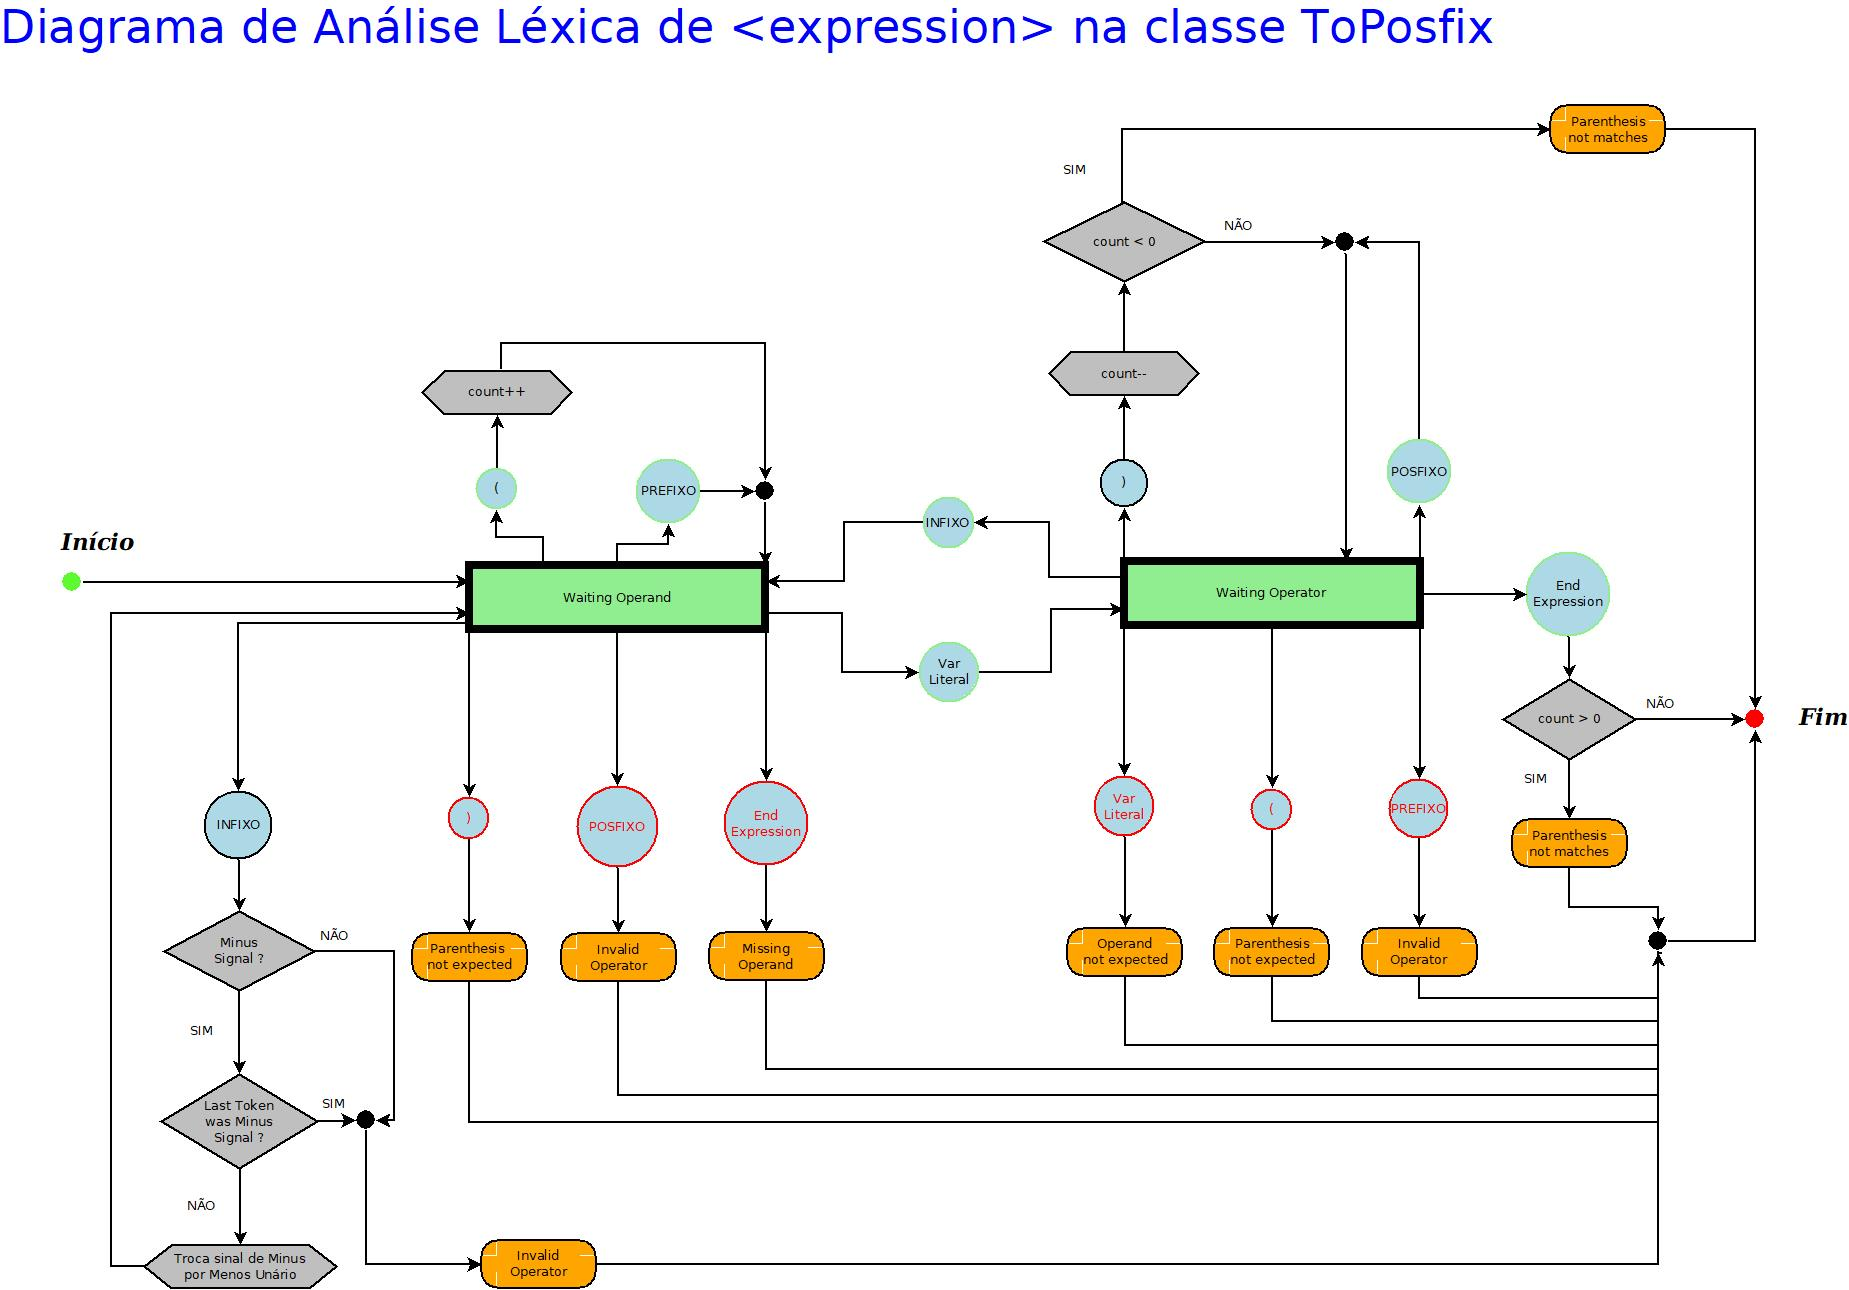
\includegraphics[height=13cm,width=20cm]{figuras/Diagrama1.jpeg}
	\caption{Diagrama da estrutura léxica de uma expressão matemática.}
	\label{figura:diagrama} 
\end{figure}

%-----------------------------------------------------------------------------
% Fim da documetação dos métodos da classe. Pula para próxima página.
%------------------------------------------------------------------------------
\newpage




%-----------------------------------------------------------------------------
% A partir dessa tag todos os capítulos são interpertados pelo Latex como 
% apêndices e indexados por letras em vez de números. Serão apêndices da parte
% onde estiverem incluídos. Neste modelo de documento as partes servem para
% documentar pacotes do projeto. Portanto cada documentação de pacote do projeto
% pode ter seus próprios apêndices.
%-----------------------------------------------------------------------------
\appendix


%\chapter{Ponha Aqui o Título do Apêndice}

%Ponha aqui o texto do apêndice.

%\newpage



\end{document}